\subsection*{Data acquisition}
We recorded the calcium activity  of dense populations of neurons in the supragranular layers of mouse primary visual cortex using fast random-access 3D scanning two-photon microscopy \cite{Stosiek:2003,Reddy:2005}   while presenting numerious repetitions of full-field drifting gratings (Fig. 1A and 1B). This technique allowed recording from a large number (150--350) of cells in a small volume of cortical tissue ($200\times200\times100$ $\mu$m$^3$) in layers 2/3 and 4. Somatic calcium signals were deconvolved using  sparse nonnegative deconvolution \cite{Vogelstein:2010} (Fig. 1C and 1D).  The average stimulus response was subtracted to remove stimulus covariance and the sample noise covariance matrix was computed (Fig. 1E).

\begin{figure}[htp]
\begin{center}
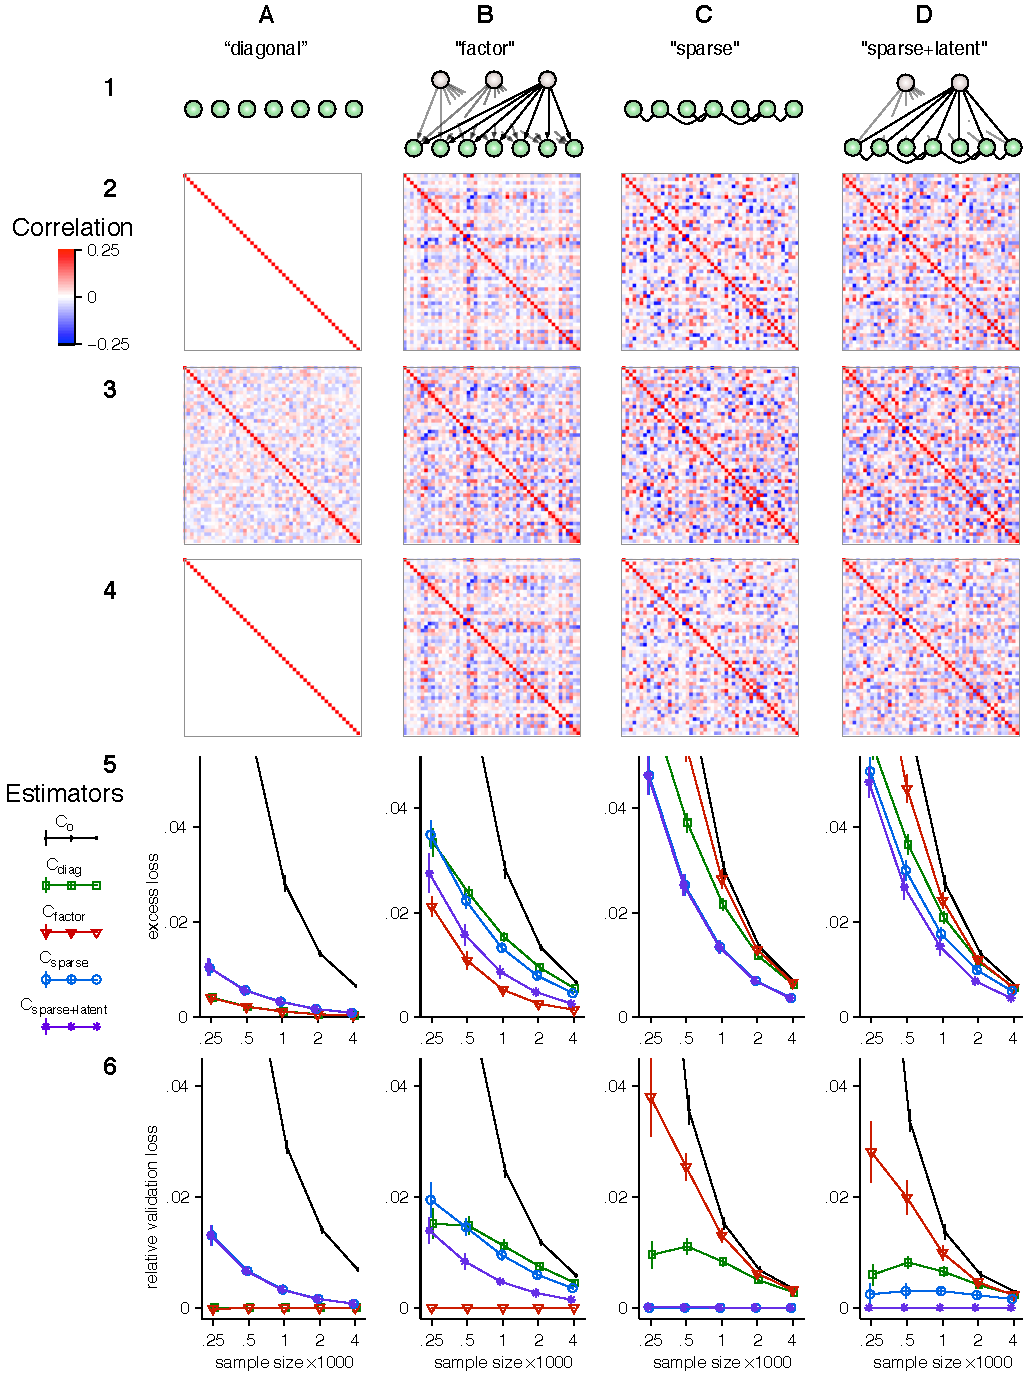
\includegraphics[width=2.5in]{figures/Figure1.pdf}
\end{center}
\caption{
{\bf Acquistion of neural population activity using two-photon fluorescence imaging of calcium signal.}  {\bf A.} Visual stimuli comprising brief (500 ms) presentatios of full-field drifting gratings separated by blank screens. {\bf B.} Two-photon fast 3D imaging of calcium signals in an awake mouse. {\bf C.} Deconvolved calcium signals. {\bf D.} The sample covariance matrix of neuronal calcium signals in 200 ms time bins. 
}
\label{Figure_label}
\end{figure}


\subsection*{Covariance estimation}
We aim to estimate the true covariance matrix $\Sigma = \mathbb E [(x-\mu)(x-\mu)^\T]$ , where $\mathbb E[\cdot]$ denotes expectation \TODO{under the true model}, $x$ denotes the $p\times 1$ vector of real-valued instanteous firing rates of $p$ neurons in a bin of duration $\Delta t$ and $\mu = \mathbb E[x]$.  For more rigourous notation, definitions, and derivations, see Appendix. 

The usual estimator of $\Sigma$ is the sample covariance matrix
\begin{equation}
\hat \Sigma_0 = \frac 1 {n-c} \sum\limits_{t=1}^n (x(t)-\mu)(x(t)-\mu)^\T 
\end{equation}
where $x(t),\;t=1,\ldots,n$ are sequential observations of population activity inferred from calcium signals. Bessel's correction $c$ makes the estimate unbiased such that $\mathbb E[\hat\Sigma_0] = \Sigma$. When observations $x(t)$ can be assumed to be independent then $c=1$; but when observations are correlated $c>1$ may be estimated from the data. 



\subsubsection*{Regularized estimates}
Although $\hat\Sigma_0$ is unbiased, it is not as close as possible to $\Sigma$.  Closer estimates can be produced by admitting a moderate amount of bias (\emph{approximation error}) in order to reduce the variance (\emph{estimation error}) of the estimate. 
\emph{Regularization} is the deliberate biasing of the estimate toward a low-dimensional target estimate in order to strike a favorable balance between bias and variance and minimize the overall expected error \cite{Bickel:2006,Ledoit:2004}.

A great variety of regularized covariance estimators can be conceived, which consistently outperform the sample covariance estimate. Regularized estimators differ from each other by the following aspects:
\begin{itemize}
\item the choice of the family of the target estimate, 
\item the choice of the specific member of the family of target estimates
\item the choice of the path from the unbiased estimate toward the chosen target
\item the distance along that path
\end{itemize}
Steps 1 and 2 produce a low-dimensional estimate. Steps 3 and 4 are often called shrinkage and allow deviations from (or distribution about) the low-dimensional estimates.

We evaluated four regularized estimators which we will denote as A, B, C, and D.  Their target estimates are graphically depicted in Figure 2. 
The green spheres represent the observed neurons. The light-colored balls represent latent units and the edges connecting them represent conditional dependencies.

\subsubsection*{Estimate A: Shrinkage toward the independent model}
In A, the target is a family of diagonal matrices 
\begin{equation}
\hat T_\alpha = (1-\alpha)(\hat\Sigma_0 \circ I) + \frac \alpha p \mbox{tr}(\hat \Sigma_0)I
\end{equation}
where $\circ$ is the entrywise product (Hadamard product). When $\alpha=0$, $\hat T_\alpha$ has the average variance along the diagonal. When $ \alpha=1$, $ \hat T_\alpha$ has empirical variances on the diagonal.

If dependencies between neurons are strictly linear, then a diagonal covariance matrix represents the case where neurons are independent, with no interactions.

The overall estimate $\hat\Sigma$ is found by linear mixing of $\hat\Sigma_0$ and $ \hat T_\alpha$ controlled by the mixing proportion $\lambda$:
\begin{equation}
\hat\Sigma = (1-\lambda)\hat\Sigma_0 + \lambda\hat T_\alpha 
\end{equation}

The hyperparameters $ \alpha$ and $ \lambda$ can be optimally selected from the training data by nested cross-validation.

\subsubsection*{Estimate B: Shrinkage toward }
In estimator B, the target is the multifactor model $ \hat T_d$ with $ d$ latent units. When all dependencies are linear, factor models correspond to mutually independent neurons each influenced by $ d$ latent units. (This is  the conventional factor analysis).

Just as in A, the overall estimate is found by linear mixing:
\begin{equation}
\hat\Sigma = (1-\lambda)\hat\Sigma_0 + \lambda\hat T_d
\end{equation}

\subsubsection*{Estimate C}
In estimate C, the target $ \hat S_\alpha$ is a matrix whose inverse is <em>sparse</em>, with a large fraction of off-diagonal elements fixed at zero. The coefficient $ \alpha$ controls the sparsity in $ \hat S_\alpha$.

In models with only linear dependencies, zeros in the inverse covariance indicate conditional independence. Thus the target estimate is depicted as the graphical model with sparse interneuronal interactions.

In practice the target $\hat S_\alpha$ is found by an $ L_1$-norm optimization technique, which combines dimensionality reduction and shrinkage into a single computationally efficient algorithm.

Just as in the previous estimators, the optimal value of the regularization parameter $ \alpha$ is determined from the data by nested cross-validation.

\subsubsection*{Estimate D}
In estimate D, the target $\hat R_{d,\alpha}$ is the matrix whose inverse is the sum of a sparse matrix $\hat S_\alpha$ and a low-rank matrix $\hat L_d$ of rank $d$.
\begin{equation}
\hat R_{d,\alpha} = (\hat S_\alpha + \hat L_d)^{-1}
\end{equation}

If all dependencies are linear, the estimate D describes a group of neurons where each interacts with a small number of latent units and a small fraction of the observed neurons. 

\subsection*{Sparse inverse covariance with a low-rank component dominates other estimators}
I computed noise covariances of population activity from 31 sites.  In each site, I compared the cross-validated performance of the covariance matrix using the Gaussian log-likelihood loss function between the trained estimate $ \hat\Sigma$ and the testing sample covariance $ \Sigma_0^\prime$:
\begin{equation}
\mathcal L(\hat\Sigma,\hat\Sigma_0^\prime) = 
\frac 1 p\left( \ln \det \hat \Sigma + \mbox{tr}(\hat \Sigma^{-1}\hat\Sigma_0^\prime) \right) 
\end{equation}

I obtained the following in figure 3.

This is the full matrix of all comparisons of the estimators.  The plots represents the histograms of the differences of the loss function between the pair of estimators for all 31 sites.  When the differences are positive, the first estimate in the title outperforms the second estimate.

Of particular interest is the first row, which shows that all regularized estimates  outperformed the sample covariance estimate.  Even more informative is the last column, which shows that estimate D (sparse+lowrank) significantly outperformed all other estimates.



